
\chapter{Planification : à partir de Microsoft Project}

\section{Hiérarchie des tâches}

Le projet est découpé en 6 tâches principales. Les tâches représentent les différentes
étapes techniques par lesquelles nous devrons passer pour développer le projet.

\begin{itemize}
\item préparation des données ;
\item stockage des données ;
\item interface avec le reconnaisseur ;
\item IHM ;
\item généralités ;
\item écriture des rapports et préparation des soutenances.
\end{itemize}

\paragraph{}

Le projet se déroule de manière parallèle en règle générale, mais chaque bloc a un fonctionnement interne séquentiel, chaque grande tâche est divisée en sous-tâches.

\paragraph{}

Tout d’abord, la partie \textbf{préparation des données} consiste à traiter les documents que l’utilisateur souhaite intégrer au logiciel pour pouvoir les découper et les mettre dans un format compatible avec la base de données.
Ensuite, la partie \textbf{stockage des données} consiste à créer une base de données (choix de la manière de stocker les données établi dans le rapport de spécifications) pour enregistrer les exemples d’apprentissage donnés par l’utilisateur et fournir une interface pour extraire ces données.
La partie interface avec le reconnaisseur consiste à fournir une interface entre le stockage et le système de reconnaissance d’écriture manuscrite.
La partie \textbf{IHM} est la partie fournissant l’interface entre le logiciel et l’utilisateur.
La partie \textbf{généralités} est une partie regroupant des travaux globaux sur le logiciel (lier les blocs entre eux, concevoir un logiciel évolutif, etc. ).
Enfin, les \textbf{rapports et soutenances} représentent une partie non négligeable du travail et surtout la partie la plus contrainte aux dates de rendus.

\section{Affectation des ressources par tâche}

Nous avons fait le choix de spécifier une ressource générique, un membre de l’équipe dans notre cas. Ce choix nous permet de garder une certaine liberté sur l’attribution des tâches durant le développement en nous permettant notamment d’affecter les tâches à un autre développeur à un instant donné. Pour le moment les développeurs ont été répartis sur chacun des blocs mais si certains blocs avancent plus vite que d’autres, il sera possible de réattribuer les rôles. Nous avons essayé de mettre au moins deux personnes par tâche pour que personne ne se retrouve seul face à un problème. Pour les tâches plus simples ou plus rapides nous n'avons mis qu'une seule personne.

\paragraph{}

Ainsi Laure et Charlotte travaillent sur la partie IHM, cette partie étant importante et comprenant suffisamment de travail pour nécessiter deux personnes dessus s’y consacrant entièrement. Timothée travaille sur la partie interface avec le reconnaisseur, cette partie est plus petite que les autres et ne nécessite qu’une personne pour être réalisée. 

\paragraph{}

La partie stockage des données est une partie différente des autres car la base de données a déjà été terminée lors du premier semestre. Ainsi, Timothée et Valentin travailleront dessus au début du second semestre pour vérifier son bon fonctionnement puis Valentin travaillera dessus seul pour terminer l’interface permettant d’y accéder. De même, le développement de la partie préparation des données a été entamé durant le premier semestre. Bien qu’étant une partie importante du projet, elle est déjà bien avancée. De fait, au début du second semestre, Enzo travaillera seul dessus, puis il sera rejoint par Valentin pour l’aider.

\paragraph{}

Cette répartition permet de répartir la charge de travail de manière équilibrée. Selon notre estimation du temps de travail pour chaque tâche, chaque membre du groupe a une charge de travail égale.

\section{Jalons}

En plus de la planification du temps de développement, nous avons intégré à notre planning des jalons qui correspondent aux dates de rendus et de soutenance. Nous avons attribué l’ensemble des ressources sur les phases de préparation des rendus et des soutenances.

\section{Diagramme de Gantt}

\begin{mdframed}[frametitle={Figure 1 : Diagramme de Gantt du projet (1/2)}, innerbottommargin=10]
\begin{center}
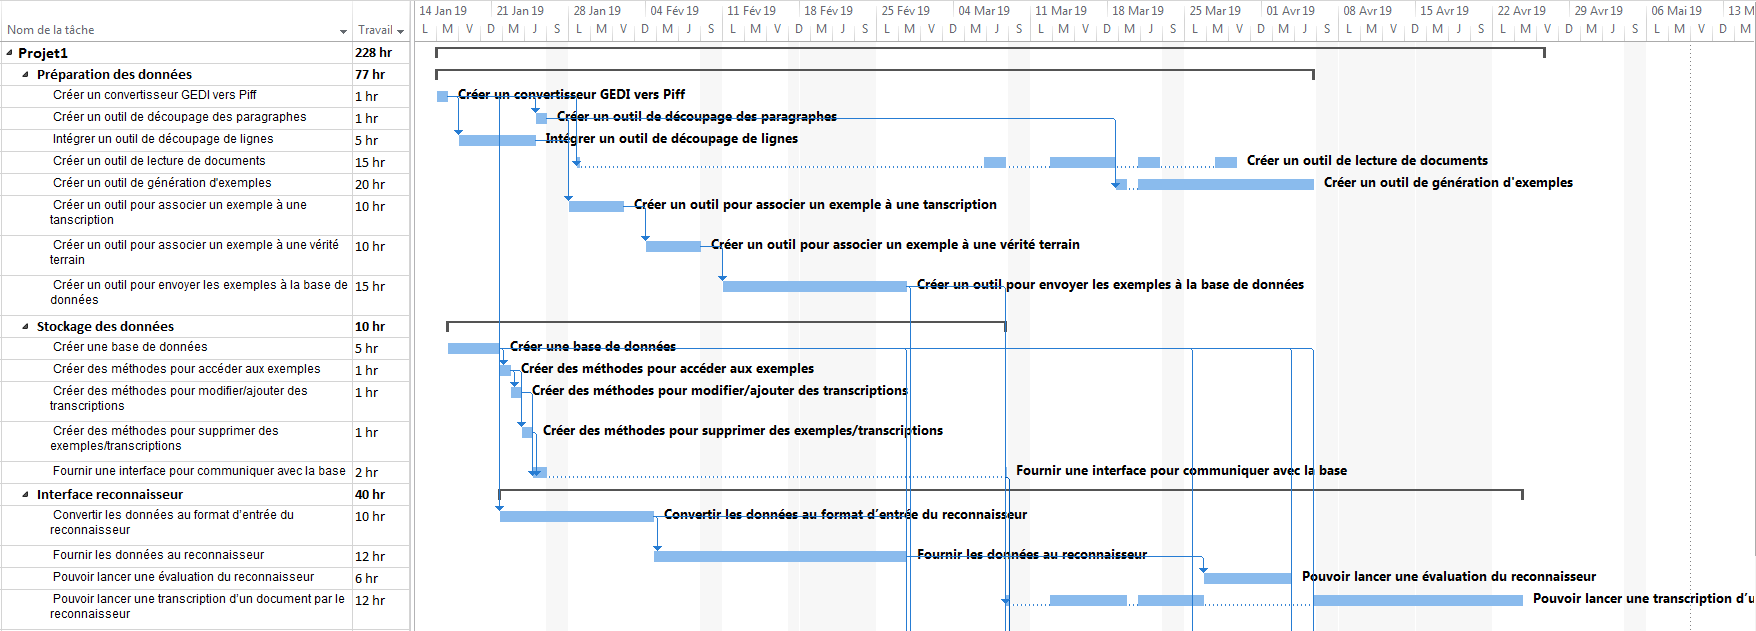
\includegraphics[scale=0.35]{gantt_V2.1.PNG}
\end{center}
\end{mdframed}

\newpage

\begin{mdframed}[frametitle={Figure 2 : Diagramme de Gantt du projet (2/2)}, innerbottommargin=10]
\begin{center}
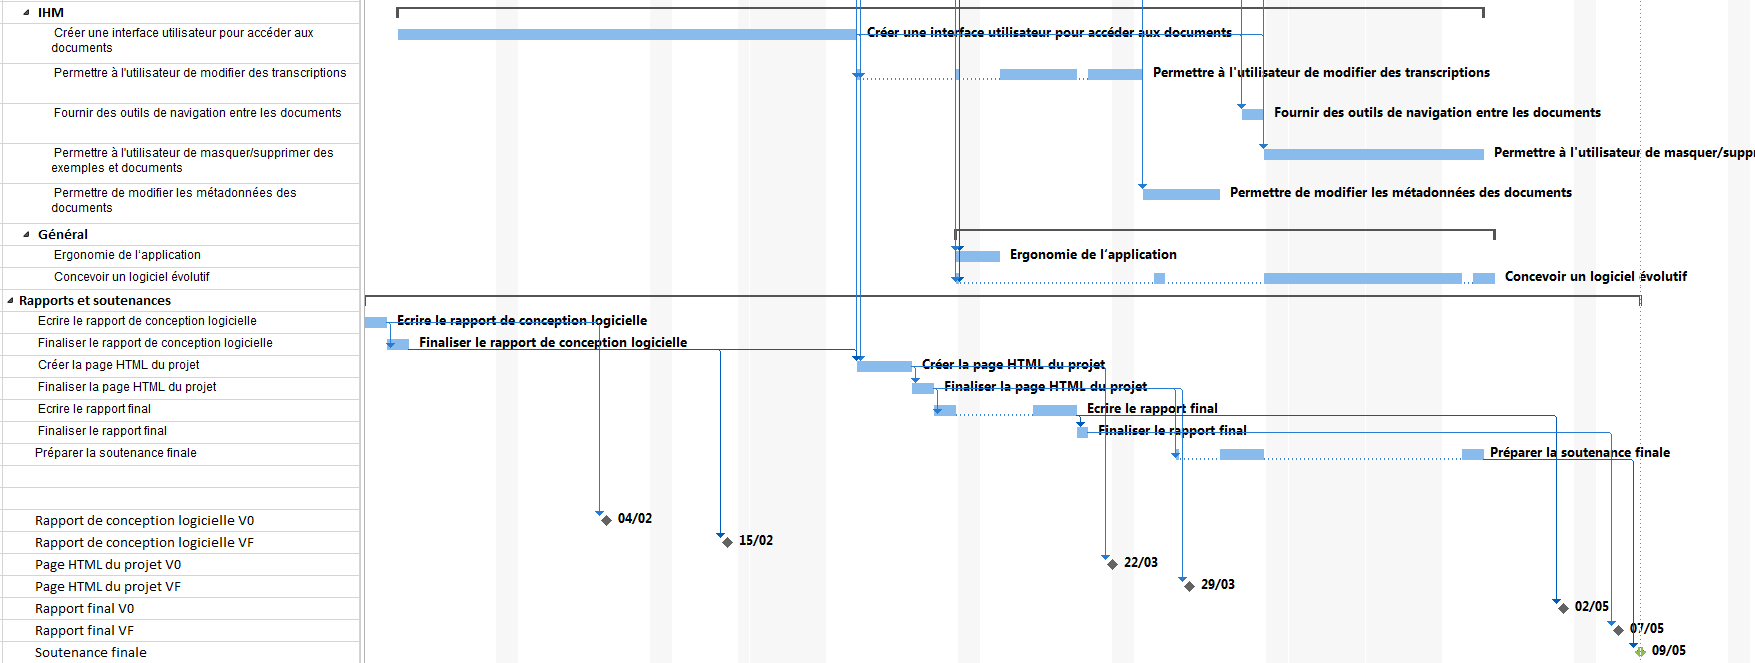
\includegraphics[scale=0.35]{gantt_V2.2.PNG}
\end{center}
\end{mdframed}

Le diagramme de Gantt ci-dessus décrit l’ensemble de la planification du projet, de la conception au rendu final en passant par la gestion de projet ou le développement de chaque itération. On y retrouve également les jalons dont nous avons parlé précédemment.

\paragraph{}
Comme dit précédemment, notre projet est consistué de deux itérations. La première itération est constitué des tâches à effectuer avant la création de la page HTML. La seconde est composée des tâches restantes.

\paragraph{}
Comme on peut le voir sur le diagramme, les quatre blocs sont biens parallèles et découpés en tâches.

















